\documentclass[11pt]{article}

    \usepackage[breakable]{tcolorbox}
    \usepackage{parskip} % Stop auto-indenting (to mimic markdown behaviour)
    
    \usepackage{iftex}
    \ifPDFTeX
    	\usepackage[T1]{fontenc}
    	\usepackage{mathpazo}
    \else
    	\usepackage{fontspec}
    \fi

    % Basic figure setup, for now with no caption control since it's done
    % automatically by Pandoc (which extracts ![](path) syntax from Markdown).
    \usepackage{graphicx}
    % Maintain compatibility with old templates. Remove in nbconvert 6.0
    \let\Oldincludegraphics\includegraphics
    % Ensure that by default, figures have no caption (until we provide a
    % proper Figure object with a Caption API and a way to capture that
    % in the conversion process - todo).
    \usepackage{caption}
    \DeclareCaptionFormat{nocaption}{}
    \captionsetup{format=nocaption,aboveskip=0pt,belowskip=0pt}

    \usepackage[Export]{adjustbox} % Used to constrain images to a maximum size
    \adjustboxset{max size={0.9\linewidth}{0.9\paperheight}}
    \usepackage{float}
    \floatplacement{figure}{H} % forces figures to be placed at the correct location
    \usepackage{xcolor} % Allow colors to be defined
    \usepackage{enumerate} % Needed for markdown enumerations to work
    \usepackage{geometry} % Used to adjust the document margins
    \usepackage{amsmath} % Equations
    \usepackage{amssymb} % Equations
    \usepackage{textcomp} % defines textquotesingle
    % Hack from http://tex.stackexchange.com/a/47451/13684:
    \AtBeginDocument{%
        \def\PYZsq{\textquotesingle}% Upright quotes in Pygmentized code
    }
    \usepackage{upquote} % Upright quotes for verbatim code
    \usepackage{eurosym} % defines \euro
    \usepackage[mathletters]{ucs} % Extended unicode (utf-8) support
    \usepackage{fancyvrb} % verbatim replacement that allows latex
    \usepackage{grffile} % extends the file name processing of package graphics 
                         % to support a larger range
    \makeatletter % fix for grffile with XeLaTeX
    \def\Gread@@xetex#1{%
      \IfFileExists{"\Gin@base".bb}%
      {\Gread@eps{\Gin@base.bb}}%
      {\Gread@@xetex@aux#1}%
    }
    \makeatother

    % The hyperref package gives us a pdf with properly built
    % internal navigation ('pdf bookmarks' for the table of contents,
    % internal cross-reference links, web links for URLs, etc.)
    \usepackage{hyperref}
    % The default LaTeX title has an obnoxious amount of whitespace. By default,
    % titling removes some of it. It also provides customization options.
    \usepackage{titling}
    \usepackage{longtable} % longtable support required by pandoc >1.10
    \usepackage{booktabs}  % table support for pandoc > 1.12.2
    \usepackage[inline]{enumitem} % IRkernel/repr support (it uses the enumerate* environment)
    \usepackage[normalem]{ulem} % ulem is needed to support strikethroughs (\sout)
                                % normalem makes italics be italics, not underlines
    \usepackage{mathrsfs}
    

    
    % Colors for the hyperref package
    \definecolor{urlcolor}{rgb}{0,.145,.698}
    \definecolor{linkcolor}{rgb}{.71,0.21,0.01}
    \definecolor{citecolor}{rgb}{.12,.54,.11}

    % ANSI colors
    \definecolor{ansi-black}{HTML}{3E424D}
    \definecolor{ansi-black-intense}{HTML}{282C36}
    \definecolor{ansi-red}{HTML}{E75C58}
    \definecolor{ansi-red-intense}{HTML}{B22B31}
    \definecolor{ansi-green}{HTML}{00A250}
    \definecolor{ansi-green-intense}{HTML}{007427}
    \definecolor{ansi-yellow}{HTML}{DDB62B}
    \definecolor{ansi-yellow-intense}{HTML}{B27D12}
    \definecolor{ansi-blue}{HTML}{208FFB}
    \definecolor{ansi-blue-intense}{HTML}{0065CA}
    \definecolor{ansi-magenta}{HTML}{D160C4}
    \definecolor{ansi-magenta-intense}{HTML}{A03196}
    \definecolor{ansi-cyan}{HTML}{60C6C8}
    \definecolor{ansi-cyan-intense}{HTML}{258F8F}
    \definecolor{ansi-white}{HTML}{C5C1B4}
    \definecolor{ansi-white-intense}{HTML}{A1A6B2}
    \definecolor{ansi-default-inverse-fg}{HTML}{FFFFFF}
    \definecolor{ansi-default-inverse-bg}{HTML}{000000}

    % commands and environments needed by pandoc snippets
    % extracted from the output of `pandoc -s`
    \providecommand{\tightlist}{%
      \setlength{\itemsep}{0pt}\setlength{\parskip}{0pt}}
    \DefineVerbatimEnvironment{Highlighting}{Verbatim}{commandchars=\\\{\}}
    % Add ',fontsize=\small' for more characters per line
    \newenvironment{Shaded}{}{}
    \newcommand{\KeywordTok}[1]{\textcolor[rgb]{0.00,0.44,0.13}{\textbf{{#1}}}}
    \newcommand{\DataTypeTok}[1]{\textcolor[rgb]{0.56,0.13,0.00}{{#1}}}
    \newcommand{\DecValTok}[1]{\textcolor[rgb]{0.25,0.63,0.44}{{#1}}}
    \newcommand{\BaseNTok}[1]{\textcolor[rgb]{0.25,0.63,0.44}{{#1}}}
    \newcommand{\FloatTok}[1]{\textcolor[rgb]{0.25,0.63,0.44}{{#1}}}
    \newcommand{\CharTok}[1]{\textcolor[rgb]{0.25,0.44,0.63}{{#1}}}
    \newcommand{\StringTok}[1]{\textcolor[rgb]{0.25,0.44,0.63}{{#1}}}
    \newcommand{\CommentTok}[1]{\textcolor[rgb]{0.38,0.63,0.69}{\textit{{#1}}}}
    \newcommand{\OtherTok}[1]{\textcolor[rgb]{0.00,0.44,0.13}{{#1}}}
    \newcommand{\AlertTok}[1]{\textcolor[rgb]{1.00,0.00,0.00}{\textbf{{#1}}}}
    \newcommand{\FunctionTok}[1]{\textcolor[rgb]{0.02,0.16,0.49}{{#1}}}
    \newcommand{\RegionMarkerTok}[1]{{#1}}
    \newcommand{\ErrorTok}[1]{\textcolor[rgb]{1.00,0.00,0.00}{\textbf{{#1}}}}
    \newcommand{\NormalTok}[1]{{#1}}
    
    % Additional commands for more recent versions of Pandoc
    \newcommand{\ConstantTok}[1]{\textcolor[rgb]{0.53,0.00,0.00}{{#1}}}
    \newcommand{\SpecialCharTok}[1]{\textcolor[rgb]{0.25,0.44,0.63}{{#1}}}
    \newcommand{\VerbatimStringTok}[1]{\textcolor[rgb]{0.25,0.44,0.63}{{#1}}}
    \newcommand{\SpecialStringTok}[1]{\textcolor[rgb]{0.73,0.40,0.53}{{#1}}}
    \newcommand{\ImportTok}[1]{{#1}}
    \newcommand{\DocumentationTok}[1]{\textcolor[rgb]{0.73,0.13,0.13}{\textit{{#1}}}}
    \newcommand{\AnnotationTok}[1]{\textcolor[rgb]{0.38,0.63,0.69}{\textbf{\textit{{#1}}}}}
    \newcommand{\CommentVarTok}[1]{\textcolor[rgb]{0.38,0.63,0.69}{\textbf{\textit{{#1}}}}}
    \newcommand{\VariableTok}[1]{\textcolor[rgb]{0.10,0.09,0.49}{{#1}}}
    \newcommand{\ControlFlowTok}[1]{\textcolor[rgb]{0.00,0.44,0.13}{\textbf{{#1}}}}
    \newcommand{\OperatorTok}[1]{\textcolor[rgb]{0.40,0.40,0.40}{{#1}}}
    \newcommand{\BuiltInTok}[1]{{#1}}
    \newcommand{\ExtensionTok}[1]{{#1}}
    \newcommand{\PreprocessorTok}[1]{\textcolor[rgb]{0.74,0.48,0.00}{{#1}}}
    \newcommand{\AttributeTok}[1]{\textcolor[rgb]{0.49,0.56,0.16}{{#1}}}
    \newcommand{\InformationTok}[1]{\textcolor[rgb]{0.38,0.63,0.69}{\textbf{\textit{{#1}}}}}
    \newcommand{\WarningTok}[1]{\textcolor[rgb]{0.38,0.63,0.69}{\textbf{\textit{{#1}}}}}
    
    
    % Define a nice break command that doesn't care if a line doesn't already
    % exist.
    \def\br{\hspace*{\fill} \\* }
    % Math Jax compatibility definitions
    \def\gt{>}
    \def\lt{<}
    \let\Oldtex\TeX
    \let\Oldlatex\LaTeX
    \renewcommand{\TeX}{\textrm{\Oldtex}}
    \renewcommand{\LaTeX}{\textrm{\Oldlatex}}
    % Document parameters
    % Document title
    \title{CAAI Data Task - Marco Gutierrez}
    
    
    
    
    
% Pygments definitions
\makeatletter
\def\PY@reset{\let\PY@it=\relax \let\PY@bf=\relax%
    \let\PY@ul=\relax \let\PY@tc=\relax%
    \let\PY@bc=\relax \let\PY@ff=\relax}
\def\PY@tok#1{\csname PY@tok@#1\endcsname}
\def\PY@toks#1+{\ifx\relax#1\empty\else%
    \PY@tok{#1}\expandafter\PY@toks\fi}
\def\PY@do#1{\PY@bc{\PY@tc{\PY@ul{%
    \PY@it{\PY@bf{\PY@ff{#1}}}}}}}
\def\PY#1#2{\PY@reset\PY@toks#1+\relax+\PY@do{#2}}

\expandafter\def\csname PY@tok@w\endcsname{\def\PY@tc##1{\textcolor[rgb]{0.73,0.73,0.73}{##1}}}
\expandafter\def\csname PY@tok@c\endcsname{\let\PY@it=\textit\def\PY@tc##1{\textcolor[rgb]{0.25,0.50,0.50}{##1}}}
\expandafter\def\csname PY@tok@cp\endcsname{\def\PY@tc##1{\textcolor[rgb]{0.74,0.48,0.00}{##1}}}
\expandafter\def\csname PY@tok@k\endcsname{\let\PY@bf=\textbf\def\PY@tc##1{\textcolor[rgb]{0.00,0.50,0.00}{##1}}}
\expandafter\def\csname PY@tok@kp\endcsname{\def\PY@tc##1{\textcolor[rgb]{0.00,0.50,0.00}{##1}}}
\expandafter\def\csname PY@tok@kt\endcsname{\def\PY@tc##1{\textcolor[rgb]{0.69,0.00,0.25}{##1}}}
\expandafter\def\csname PY@tok@o\endcsname{\def\PY@tc##1{\textcolor[rgb]{0.40,0.40,0.40}{##1}}}
\expandafter\def\csname PY@tok@ow\endcsname{\let\PY@bf=\textbf\def\PY@tc##1{\textcolor[rgb]{0.67,0.13,1.00}{##1}}}
\expandafter\def\csname PY@tok@nb\endcsname{\def\PY@tc##1{\textcolor[rgb]{0.00,0.50,0.00}{##1}}}
\expandafter\def\csname PY@tok@nf\endcsname{\def\PY@tc##1{\textcolor[rgb]{0.00,0.00,1.00}{##1}}}
\expandafter\def\csname PY@tok@nc\endcsname{\let\PY@bf=\textbf\def\PY@tc##1{\textcolor[rgb]{0.00,0.00,1.00}{##1}}}
\expandafter\def\csname PY@tok@nn\endcsname{\let\PY@bf=\textbf\def\PY@tc##1{\textcolor[rgb]{0.00,0.00,1.00}{##1}}}
\expandafter\def\csname PY@tok@ne\endcsname{\let\PY@bf=\textbf\def\PY@tc##1{\textcolor[rgb]{0.82,0.25,0.23}{##1}}}
\expandafter\def\csname PY@tok@nv\endcsname{\def\PY@tc##1{\textcolor[rgb]{0.10,0.09,0.49}{##1}}}
\expandafter\def\csname PY@tok@no\endcsname{\def\PY@tc##1{\textcolor[rgb]{0.53,0.00,0.00}{##1}}}
\expandafter\def\csname PY@tok@nl\endcsname{\def\PY@tc##1{\textcolor[rgb]{0.63,0.63,0.00}{##1}}}
\expandafter\def\csname PY@tok@ni\endcsname{\let\PY@bf=\textbf\def\PY@tc##1{\textcolor[rgb]{0.60,0.60,0.60}{##1}}}
\expandafter\def\csname PY@tok@na\endcsname{\def\PY@tc##1{\textcolor[rgb]{0.49,0.56,0.16}{##1}}}
\expandafter\def\csname PY@tok@nt\endcsname{\let\PY@bf=\textbf\def\PY@tc##1{\textcolor[rgb]{0.00,0.50,0.00}{##1}}}
\expandafter\def\csname PY@tok@nd\endcsname{\def\PY@tc##1{\textcolor[rgb]{0.67,0.13,1.00}{##1}}}
\expandafter\def\csname PY@tok@s\endcsname{\def\PY@tc##1{\textcolor[rgb]{0.73,0.13,0.13}{##1}}}
\expandafter\def\csname PY@tok@sd\endcsname{\let\PY@it=\textit\def\PY@tc##1{\textcolor[rgb]{0.73,0.13,0.13}{##1}}}
\expandafter\def\csname PY@tok@si\endcsname{\let\PY@bf=\textbf\def\PY@tc##1{\textcolor[rgb]{0.73,0.40,0.53}{##1}}}
\expandafter\def\csname PY@tok@se\endcsname{\let\PY@bf=\textbf\def\PY@tc##1{\textcolor[rgb]{0.73,0.40,0.13}{##1}}}
\expandafter\def\csname PY@tok@sr\endcsname{\def\PY@tc##1{\textcolor[rgb]{0.73,0.40,0.53}{##1}}}
\expandafter\def\csname PY@tok@ss\endcsname{\def\PY@tc##1{\textcolor[rgb]{0.10,0.09,0.49}{##1}}}
\expandafter\def\csname PY@tok@sx\endcsname{\def\PY@tc##1{\textcolor[rgb]{0.00,0.50,0.00}{##1}}}
\expandafter\def\csname PY@tok@m\endcsname{\def\PY@tc##1{\textcolor[rgb]{0.40,0.40,0.40}{##1}}}
\expandafter\def\csname PY@tok@gh\endcsname{\let\PY@bf=\textbf\def\PY@tc##1{\textcolor[rgb]{0.00,0.00,0.50}{##1}}}
\expandafter\def\csname PY@tok@gu\endcsname{\let\PY@bf=\textbf\def\PY@tc##1{\textcolor[rgb]{0.50,0.00,0.50}{##1}}}
\expandafter\def\csname PY@tok@gd\endcsname{\def\PY@tc##1{\textcolor[rgb]{0.63,0.00,0.00}{##1}}}
\expandafter\def\csname PY@tok@gi\endcsname{\def\PY@tc##1{\textcolor[rgb]{0.00,0.63,0.00}{##1}}}
\expandafter\def\csname PY@tok@gr\endcsname{\def\PY@tc##1{\textcolor[rgb]{1.00,0.00,0.00}{##1}}}
\expandafter\def\csname PY@tok@ge\endcsname{\let\PY@it=\textit}
\expandafter\def\csname PY@tok@gs\endcsname{\let\PY@bf=\textbf}
\expandafter\def\csname PY@tok@gp\endcsname{\let\PY@bf=\textbf\def\PY@tc##1{\textcolor[rgb]{0.00,0.00,0.50}{##1}}}
\expandafter\def\csname PY@tok@go\endcsname{\def\PY@tc##1{\textcolor[rgb]{0.53,0.53,0.53}{##1}}}
\expandafter\def\csname PY@tok@gt\endcsname{\def\PY@tc##1{\textcolor[rgb]{0.00,0.27,0.87}{##1}}}
\expandafter\def\csname PY@tok@err\endcsname{\def\PY@bc##1{\setlength{\fboxsep}{0pt}\fcolorbox[rgb]{1.00,0.00,0.00}{1,1,1}{\strut ##1}}}
\expandafter\def\csname PY@tok@kc\endcsname{\let\PY@bf=\textbf\def\PY@tc##1{\textcolor[rgb]{0.00,0.50,0.00}{##1}}}
\expandafter\def\csname PY@tok@kd\endcsname{\let\PY@bf=\textbf\def\PY@tc##1{\textcolor[rgb]{0.00,0.50,0.00}{##1}}}
\expandafter\def\csname PY@tok@kn\endcsname{\let\PY@bf=\textbf\def\PY@tc##1{\textcolor[rgb]{0.00,0.50,0.00}{##1}}}
\expandafter\def\csname PY@tok@kr\endcsname{\let\PY@bf=\textbf\def\PY@tc##1{\textcolor[rgb]{0.00,0.50,0.00}{##1}}}
\expandafter\def\csname PY@tok@bp\endcsname{\def\PY@tc##1{\textcolor[rgb]{0.00,0.50,0.00}{##1}}}
\expandafter\def\csname PY@tok@fm\endcsname{\def\PY@tc##1{\textcolor[rgb]{0.00,0.00,1.00}{##1}}}
\expandafter\def\csname PY@tok@vc\endcsname{\def\PY@tc##1{\textcolor[rgb]{0.10,0.09,0.49}{##1}}}
\expandafter\def\csname PY@tok@vg\endcsname{\def\PY@tc##1{\textcolor[rgb]{0.10,0.09,0.49}{##1}}}
\expandafter\def\csname PY@tok@vi\endcsname{\def\PY@tc##1{\textcolor[rgb]{0.10,0.09,0.49}{##1}}}
\expandafter\def\csname PY@tok@vm\endcsname{\def\PY@tc##1{\textcolor[rgb]{0.10,0.09,0.49}{##1}}}
\expandafter\def\csname PY@tok@sa\endcsname{\def\PY@tc##1{\textcolor[rgb]{0.73,0.13,0.13}{##1}}}
\expandafter\def\csname PY@tok@sb\endcsname{\def\PY@tc##1{\textcolor[rgb]{0.73,0.13,0.13}{##1}}}
\expandafter\def\csname PY@tok@sc\endcsname{\def\PY@tc##1{\textcolor[rgb]{0.73,0.13,0.13}{##1}}}
\expandafter\def\csname PY@tok@dl\endcsname{\def\PY@tc##1{\textcolor[rgb]{0.73,0.13,0.13}{##1}}}
\expandafter\def\csname PY@tok@s2\endcsname{\def\PY@tc##1{\textcolor[rgb]{0.73,0.13,0.13}{##1}}}
\expandafter\def\csname PY@tok@sh\endcsname{\def\PY@tc##1{\textcolor[rgb]{0.73,0.13,0.13}{##1}}}
\expandafter\def\csname PY@tok@s1\endcsname{\def\PY@tc##1{\textcolor[rgb]{0.73,0.13,0.13}{##1}}}
\expandafter\def\csname PY@tok@mb\endcsname{\def\PY@tc##1{\textcolor[rgb]{0.40,0.40,0.40}{##1}}}
\expandafter\def\csname PY@tok@mf\endcsname{\def\PY@tc##1{\textcolor[rgb]{0.40,0.40,0.40}{##1}}}
\expandafter\def\csname PY@tok@mh\endcsname{\def\PY@tc##1{\textcolor[rgb]{0.40,0.40,0.40}{##1}}}
\expandafter\def\csname PY@tok@mi\endcsname{\def\PY@tc##1{\textcolor[rgb]{0.40,0.40,0.40}{##1}}}
\expandafter\def\csname PY@tok@il\endcsname{\def\PY@tc##1{\textcolor[rgb]{0.40,0.40,0.40}{##1}}}
\expandafter\def\csname PY@tok@mo\endcsname{\def\PY@tc##1{\textcolor[rgb]{0.40,0.40,0.40}{##1}}}
\expandafter\def\csname PY@tok@ch\endcsname{\let\PY@it=\textit\def\PY@tc##1{\textcolor[rgb]{0.25,0.50,0.50}{##1}}}
\expandafter\def\csname PY@tok@cm\endcsname{\let\PY@it=\textit\def\PY@tc##1{\textcolor[rgb]{0.25,0.50,0.50}{##1}}}
\expandafter\def\csname PY@tok@cpf\endcsname{\let\PY@it=\textit\def\PY@tc##1{\textcolor[rgb]{0.25,0.50,0.50}{##1}}}
\expandafter\def\csname PY@tok@c1\endcsname{\let\PY@it=\textit\def\PY@tc##1{\textcolor[rgb]{0.25,0.50,0.50}{##1}}}
\expandafter\def\csname PY@tok@cs\endcsname{\let\PY@it=\textit\def\PY@tc##1{\textcolor[rgb]{0.25,0.50,0.50}{##1}}}

\def\PYZbs{\char`\\}
\def\PYZus{\char`\_}
\def\PYZob{\char`\{}
\def\PYZcb{\char`\}}
\def\PYZca{\char`\^}
\def\PYZam{\char`\&}
\def\PYZlt{\char`\<}
\def\PYZgt{\char`\>}
\def\PYZsh{\char`\#}
\def\PYZpc{\char`\%}
\def\PYZdl{\char`\$}
\def\PYZhy{\char`\-}
\def\PYZsq{\char`\'}
\def\PYZdq{\char`\"}
\def\PYZti{\char`\~}
% for compatibility with earlier versions
\def\PYZat{@}
\def\PYZlb{[}
\def\PYZrb{]}
\makeatother


    % For linebreaks inside Verbatim environment from package fancyvrb. 
    \makeatletter
        \newbox\Wrappedcontinuationbox 
        \newbox\Wrappedvisiblespacebox 
        \newcommand*\Wrappedvisiblespace {\textcolor{red}{\textvisiblespace}} 
        \newcommand*\Wrappedcontinuationsymbol {\textcolor{red}{\llap{\tiny$\m@th\hookrightarrow$}}} 
        \newcommand*\Wrappedcontinuationindent {3ex } 
        \newcommand*\Wrappedafterbreak {\kern\Wrappedcontinuationindent\copy\Wrappedcontinuationbox} 
        % Take advantage of the already applied Pygments mark-up to insert 
        % potential linebreaks for TeX processing. 
        %        {, <, #, %, $, ' and ": go to next line. 
        %        _, }, ^, &, >, - and ~: stay at end of broken line. 
        % Use of \textquotesingle for straight quote. 
        \newcommand*\Wrappedbreaksatspecials {% 
            \def\PYGZus{\discretionary{\char`\_}{\Wrappedafterbreak}{\char`\_}}% 
            \def\PYGZob{\discretionary{}{\Wrappedafterbreak\char`\{}{\char`\{}}% 
            \def\PYGZcb{\discretionary{\char`\}}{\Wrappedafterbreak}{\char`\}}}% 
            \def\PYGZca{\discretionary{\char`\^}{\Wrappedafterbreak}{\char`\^}}% 
            \def\PYGZam{\discretionary{\char`\&}{\Wrappedafterbreak}{\char`\&}}% 
            \def\PYGZlt{\discretionary{}{\Wrappedafterbreak\char`\<}{\char`\<}}% 
            \def\PYGZgt{\discretionary{\char`\>}{\Wrappedafterbreak}{\char`\>}}% 
            \def\PYGZsh{\discretionary{}{\Wrappedafterbreak\char`\#}{\char`\#}}% 
            \def\PYGZpc{\discretionary{}{\Wrappedafterbreak\char`\%}{\char`\%}}% 
            \def\PYGZdl{\discretionary{}{\Wrappedafterbreak\char`\$}{\char`\$}}% 
            \def\PYGZhy{\discretionary{\char`\-}{\Wrappedafterbreak}{\char`\-}}% 
            \def\PYGZsq{\discretionary{}{\Wrappedafterbreak\textquotesingle}{\textquotesingle}}% 
            \def\PYGZdq{\discretionary{}{\Wrappedafterbreak\char`\"}{\char`\"}}% 
            \def\PYGZti{\discretionary{\char`\~}{\Wrappedafterbreak}{\char`\~}}% 
        } 
        % Some characters . , ; ? ! / are not pygmentized. 
        % This macro makes them "active" and they will insert potential linebreaks 
        \newcommand*\Wrappedbreaksatpunct {% 
            \lccode`\~`\.\lowercase{\def~}{\discretionary{\hbox{\char`\.}}{\Wrappedafterbreak}{\hbox{\char`\.}}}% 
            \lccode`\~`\,\lowercase{\def~}{\discretionary{\hbox{\char`\,}}{\Wrappedafterbreak}{\hbox{\char`\,}}}% 
            \lccode`\~`\;\lowercase{\def~}{\discretionary{\hbox{\char`\;}}{\Wrappedafterbreak}{\hbox{\char`\;}}}% 
            \lccode`\~`\:\lowercase{\def~}{\discretionary{\hbox{\char`\:}}{\Wrappedafterbreak}{\hbox{\char`\:}}}% 
            \lccode`\~`\?\lowercase{\def~}{\discretionary{\hbox{\char`\?}}{\Wrappedafterbreak}{\hbox{\char`\?}}}% 
            \lccode`\~`\!\lowercase{\def~}{\discretionary{\hbox{\char`\!}}{\Wrappedafterbreak}{\hbox{\char`\!}}}% 
            \lccode`\~`\/\lowercase{\def~}{\discretionary{\hbox{\char`\/}}{\Wrappedafterbreak}{\hbox{\char`\/}}}% 
            \catcode`\.\active
            \catcode`\,\active 
            \catcode`\;\active
            \catcode`\:\active
            \catcode`\?\active
            \catcode`\!\active
            \catcode`\/\active 
            \lccode`\~`\~ 	
        }
    \makeatother

    \let\OriginalVerbatim=\Verbatim
    \makeatletter
    \renewcommand{\Verbatim}[1][1]{%
        %\parskip\z@skip
        \sbox\Wrappedcontinuationbox {\Wrappedcontinuationsymbol}%
        \sbox\Wrappedvisiblespacebox {\FV@SetupFont\Wrappedvisiblespace}%
        \def\FancyVerbFormatLine ##1{\hsize\linewidth
            \vtop{\raggedright\hyphenpenalty\z@\exhyphenpenalty\z@
                \doublehyphendemerits\z@\finalhyphendemerits\z@
                \strut ##1\strut}%
        }%
        % If the linebreak is at a space, the latter will be displayed as visible
        % space at end of first line, and a continuation symbol starts next line.
        % Stretch/shrink are however usually zero for typewriter font.
        \def\FV@Space {%
            \nobreak\hskip\z@ plus\fontdimen3\font minus\fontdimen4\font
            \discretionary{\copy\Wrappedvisiblespacebox}{\Wrappedafterbreak}
            {\kern\fontdimen2\font}%
        }%
        
        % Allow breaks at special characters using \PYG... macros.
        \Wrappedbreaksatspecials
        % Breaks at punctuation characters . , ; ? ! and / need catcode=\active 	
        \OriginalVerbatim[#1,codes*=\Wrappedbreaksatpunct]%
    }
    \makeatother

    % Exact colors from NB
    \definecolor{incolor}{HTML}{303F9F}
    \definecolor{outcolor}{HTML}{D84315}
    \definecolor{cellborder}{HTML}{CFCFCF}
    \definecolor{cellbackground}{HTML}{F7F7F7}
    
    % prompt
    \makeatletter
    \newcommand{\boxspacing}{\kern\kvtcb@left@rule\kern\kvtcb@boxsep}
    \makeatother
    \newcommand{\prompt}[4]{
        \ttfamily\llap{{\color{#2}[#3]:\hspace{3pt}#4}}\vspace{-\baselineskip}
    }
    

    
    % Prevent overflowing lines due to hard-to-break entities
    \sloppy 
    % Setup hyperref package
    \hypersetup{
      breaklinks=true,  % so long urls are correctly broken across lines
      colorlinks=true,
      urlcolor=urlcolor,
      linkcolor=linkcolor,
      citecolor=citecolor,
      }
    % Slightly bigger margins than the latex defaults
    
    \geometry{verbose,tmargin=1in,bmargin=1in,lmargin=1in,rmargin=1in}
    
    

\begin{document}
    
    \maketitle
    
    

    
    \hypertarget{importing-main-libraries}{%
\subsubsection*{Importing main
libraries}\label{importing-main-libraries}}

    \begin{tcolorbox}[breakable, size=fbox, boxrule=1pt, pad at break*=1mm,colback=cellbackground, colframe=cellborder]
\prompt{In}{incolor}{53}{\boxspacing}
\begin{Verbatim}[commandchars=\\\{\}]
\PY{o}{\PYZpc{}}\PY{k}{matplotlib} notebook
\PY{k+kn}{import} \PY{n+nn}{matplotlib} \PY{k}{as} \PY{n+nn}{mpl}
\PY{k+kn}{import} \PY{n+nn}{matplotlib}\PY{n+nn}{.}\PY{n+nn}{patches} \PY{k}{as} \PY{n+nn}{mpatches}
\PY{k+kn}{import} \PY{n+nn}{matplotlib}\PY{n+nn}{.}\PY{n+nn}{pyplot} \PY{k}{as} \PY{n+nn}{plt}
\PY{k+kn}{import} \PY{n+nn}{numpy} \PY{k}{as} \PY{n+nn}{np}
\PY{k+kn}{from} \PY{n+nn}{scipy}\PY{n+nn}{.}\PY{n+nn}{io} \PY{k+kn}{import} \PY{n}{loadmat}
\PY{k+kn}{import} \PY{n+nn}{pandas} \PY{k}{as} \PY{n+nn}{pd}
\PY{k+kn}{import} \PY{n+nn}{datetime} \PY{k}{as} \PY{n+nn}{dt}
\end{Verbatim}
\end{tcolorbox}

    \hypertarget{question-1-finding-the-imdb-wiki-dataset}{%
\section*{Question 1: Finding the IMDB-WIKI
Dataset}\label{question-1-finding-the-imdb-wiki-dataset}}

    This dataset can be found
\href{https://data.vision.ee.ethz.ch/cvl/rrothe/imdb-wiki/}{here}.
However, this notebook only works with its
\href{https://data.vision.ee.ethz.ch/cvl/rrothe/imdb-wiki/static/imdb_meta.tar}{metadata}

    \begin{tcolorbox}[breakable, size=fbox, boxrule=1pt, pad at break*=1mm,colback=cellbackground, colframe=cellborder]
\prompt{In}{incolor}{56}{\boxspacing}
\begin{Verbatim}[commandchars=\\\{\}]
\PY{n}{data} \PY{o}{=} \PY{n}{loadmat}\PY{p}{(}\PY{l+s+s2}{\PYZdq{}}\PY{l+s+s2}{Datasets}\PY{l+s+s2}{\PYZbs{}}\PY{l+s+s2}{imdb}\PY{l+s+s2}{\PYZbs{}}\PY{l+s+s2}{imdb.mat}\PY{l+s+s2}{\PYZdq{}}\PY{p}{)} \PY{c+c1}{\PYZsh{} loading the database metadata}
\end{Verbatim}
\end{tcolorbox}

    \begin{tcolorbox}[breakable, size=fbox, boxrule=1pt, pad at break*=1mm,colback=cellbackground, colframe=cellborder]
\prompt{In}{incolor}{3}{\boxspacing}
\begin{Verbatim}[commandchars=\\\{\}]
\PY{n}{data} \PY{c+c1}{\PYZsh{} displaying the raw dataset}
\end{Verbatim}
\end{tcolorbox}

            \begin{tcolorbox}[breakable, size=fbox, boxrule=.5pt, pad at break*=1mm, opacityfill=0]
\prompt{Out}{outcolor}{3}{\boxspacing}
\begin{Verbatim}[commandchars=\\\{\}]
\{'\_\_header\_\_': b'MATLAB 5.0 MAT-file, Platform: GLNXA64, Created on: Sun Jan 17
11:30:27 2016',
 '\_\_version\_\_': '1.0',
 '\_\_globals\_\_': [],
 'imdb': array([[(array([[693726, 693726, 693726, {\ldots}, 726831, 726831,
726831]]), array([[1968, 1970, 1968, {\ldots}, 2011, 2011, 2011]], dtype=uint16),
array([[array(['01/nm0000001\_rm124825600\_1899-5-10\_1968.jpg'], dtype='<U43'),
         array(['01/nm0000001\_rm3343756032\_1899-5-10\_1970.jpg'], dtype='<U44'),
         array(['01/nm0000001\_rm577153792\_1899-5-10\_1968.jpg'], dtype='<U43'),
         {\ldots},
         array(['08/nm3994408\_rm926592512\_1989-12-29\_2011.jpg'], dtype='<U44'),
         array(['08/nm3994408\_rm943369728\_1989-12-29\_2011.jpg'], dtype='<U44'),
         array(['08/nm3994408\_rm976924160\_1989-12-29\_2011.jpg'],
dtype='<U44')]],
       dtype=object), array([[1., 1., 1., {\ldots}, 0., 0., 0.]]),
array([[array(['Fred Astaire'], dtype='<U12'),
         array(['Fred Astaire'], dtype='<U12'),
         array(['Fred Astaire'], dtype='<U12'), {\ldots},
         array(['Jane Levy'], dtype='<U9'),
         array(['Jane Levy'], dtype='<U9'),
         array(['Jane Levy'], dtype='<U9')]], dtype=object),
array([[array([[1072.926,  161.838, 1214.784,  303.696]]),
         array([[477.184, 100.352, 622.592, 245.76 ]]),
         array([[114.96964309, 114.96964309, 451.68657236, 451.68657236]]),
         {\ldots}, array([[  1,   1, 453, 640]], dtype=uint16),
         array([[144.75225472, 126.76472288, 305.78804127, 287.80050943]]),
         array([[457.524,  41.748, 518.016, 102.24 ]])]], dtype=object),
array([[1.45969291, 2.5431976 , 3.45557949, {\ldots},       -inf, 4.45072452,
         2.13350269]]), array([[1.11897336, 1.85200773, 2.98566022, {\ldots},
nan,        nan,
                nan]]), array([[array(["'Lee' George Quinones"], dtype='<U21'),
         array(["'Weird Al' Yankovic"], dtype='<U19'),
         array(['2 Chainz'], dtype='<U8'), {\ldots},
         array(['Éric Caravaca'], dtype='<U13'),
         array(['Ólafur Darri Ólafsson'], dtype='<U21'),
         array(['Óscar Jaenada'], dtype='<U13')]], dtype=object), array([[6488,
6488, 6488, {\ldots}, 8410, 8410, 8410]], dtype=uint16))]],
       dtype=[('dob', 'O'), ('photo\_taken', 'O'), ('full\_path', 'O'), ('gender',
'O'), ('name', 'O'), ('face\_location', 'O'), ('face\_score', 'O'),
('second\_face\_score', 'O'), ('celeb\_names', 'O'), ('celeb\_id', 'O')])\}
\end{Verbatim}
\end{tcolorbox}
        
    \hypertarget{reading-our-dataset}{%
\section*{Reading our dataset}\label{reading-our-dataset}}

    As this dataset is in a \texttt{.mat} format, it's required to convert
it into a format Python can understand

    \hypertarget{obtaining-an-identifier-of-each-observation}{%
\subsection*{Obtaining an identifier of each
observation}\label{obtaining-an-identifier-of-each-observation}}

    \begin{tcolorbox}[breakable, size=fbox, boxrule=1pt, pad at break*=1mm,colback=cellbackground, colframe=cellborder]
\prompt{In}{incolor}{4}{\boxspacing}
\begin{Verbatim}[commandchars=\\\{\}]
\PY{n}{identifier} \PY{o}{=} \PY{n}{data}\PY{p}{[}\PY{l+s+s1}{\PYZsq{}}\PY{l+s+s1}{imdb}\PY{l+s+s1}{\PYZsq{}}\PY{p}{]}
\PY{n}{id\PYZus{}type} \PY{o}{=} \PY{n}{identifier}\PY{o}{.}\PY{n}{dtype}
\end{Verbatim}
\end{tcolorbox}

    \hypertarget{turning-the-dataset-into-a-pandas-dataframe}{%
\subsection*{Turning the dataset into a Panda's
dataframe}\label{turning-the-dataset-into-a-pandas-dataframe}}

    \begin{tcolorbox}[breakable, size=fbox, boxrule=1pt, pad at break*=1mm,colback=cellbackground, colframe=cellborder]
\prompt{In}{incolor}{5}{\boxspacing}
\begin{Verbatim}[commandchars=\\\{\}]
\PY{n}{ndata} \PY{o}{=} \PY{p}{\PYZob{}}\PY{n}{n}\PY{p}{:} \PY{n}{identifier}\PY{p}{[}\PY{n}{n}\PY{p}{]}\PY{p}{[}\PY{l+m+mi}{0}\PY{p}{,} \PY{l+m+mi}{0}\PY{p}{]} \PY{k}{for} \PY{n}{n} \PY{o+ow}{in} \PY{n}{id\PYZus{}type}\PY{o}{.}\PY{n}{names}\PY{p}{\PYZcb{}} \PY{c+c1}{\PYZsh{} creating a dictionary with the dataset information in original format}
\PY{n}{new\PYZus{}ndata} \PY{o}{=} \PY{p}{\PYZob{}}\PY{p}{\PYZcb{}} \PY{c+c1}{\PYZsh{} dictionary for storing the column values as an array per column}

\PY{k}{for} \PY{n}{key}\PY{p}{,} \PY{n}{value} \PY{o+ow}{in} \PY{n}{ndata}\PY{o}{.}\PY{n}{items}\PY{p}{(}\PY{p}{)}\PY{p}{:}
    \PY{n}{new\PYZus{}ndata}\PY{p}{[}\PY{n}{key}\PY{p}{]} \PY{o}{=} \PY{n}{value}\PY{p}{[}\PY{l+m+mi}{0}\PY{p}{]} \PY{c+c1}{\PYZsh{} assign to each column key its respective values}

\PY{n}{new\PYZus{}ndata}\PY{o}{.}\PY{n}{pop}\PY{p}{(}\PY{l+s+s1}{\PYZsq{}}\PY{l+s+s1}{celeb\PYZus{}names}\PY{l+s+s1}{\PYZsq{}}\PY{p}{,} \PY{k+kc}{None}\PY{p}{)} \PY{c+c1}{\PYZsh{} erasing column as it\PYZsq{}s the only case with a different number of observations than the rest}
\PY{n}{df} \PY{o}{=} \PY{n}{pd}\PY{o}{.}\PY{n}{DataFrame}\PY{p}{(}\PY{n}{new\PYZus{}ndata}\PY{p}{)}
\end{Verbatim}
\end{tcolorbox}

    \begin{tcolorbox}[breakable, size=fbox, boxrule=1pt, pad at break*=1mm,colback=cellbackground, colframe=cellborder]
\prompt{In}{incolor}{6}{\boxspacing}
\begin{Verbatim}[commandchars=\\\{\}]
\PY{n}{df} \PY{c+c1}{\PYZsh{} displaying the dataframe}
\end{Verbatim}
\end{tcolorbox}

            \begin{tcolorbox}[breakable, size=fbox, boxrule=.5pt, pad at break*=1mm, opacityfill=0]
\prompt{Out}{outcolor}{6}{\boxspacing}
\begin{Verbatim}[commandchars=\\\{\}]
           dob  photo\_taken                                       full\_path  \textbackslash{}
0       693726         1968   [01/nm0000001\_rm124825600\_1899-5-10\_1968.jpg]
1       693726         1970  [01/nm0000001\_rm3343756032\_1899-5-10\_1970.jpg]
2       693726         1968   [01/nm0000001\_rm577153792\_1899-5-10\_1968.jpg]
3       693726         1968   [01/nm0000001\_rm946909184\_1899-5-10\_1968.jpg]
4       693726         1968   [01/nm0000001\_rm980463616\_1899-5-10\_1968.jpg]
{\ldots}        {\ldots}          {\ldots}                                             {\ldots}
460718  726831         2011  [08/nm3994408\_rm761245696\_1989-12-29\_2011.jpg]
460719  726831         2011  [08/nm3994408\_rm784182528\_1989-12-29\_2011.jpg]
460720  726831         2011  [08/nm3994408\_rm926592512\_1989-12-29\_2011.jpg]
460721  726831         2011  [08/nm3994408\_rm943369728\_1989-12-29\_2011.jpg]
460722  726831         2011  [08/nm3994408\_rm976924160\_1989-12-29\_2011.jpg]

        gender            name  \textbackslash{}
0          1.0  [Fred Astaire]
1          1.0  [Fred Astaire]
2          1.0  [Fred Astaire]
3          1.0  [Fred Astaire]
4          1.0  [Fred Astaire]
{\ldots}        {\ldots}             {\ldots}
460718     0.0     [Jane Levy]
460719     0.0     [Jane Levy]
460720     0.0     [Jane Levy]
460721     0.0     [Jane Levy]
460722     0.0     [Jane Levy]

                                            face\_location  face\_score  \textbackslash{}
0       [[1072.926, 161.838, 1214.7839999999999, 303.6{\ldots}    1.459693
1                   [[477.184, 100.352, 622.592, 245.76]]    2.543198
2       [[114.96964308962852, 114.96964308962852, 451{\ldots}    3.455579
3       [[622.8855056426588, 424.21750383700805, 844.3{\ldots}    1.872117
4       [[1013.8590023603723, 233.8820422075853, 1201{\ldots}    1.158766
{\ldots}                                                   {\ldots}         {\ldots}
460718  [[453.8981431333457, 77.96623712908011, 539.79{\ldots}    3.845884
460719                                 [[1, 1, 426, 640]]        -inf
460720                                 [[1, 1, 453, 640]]        -inf
460721  [[144.75225471724875, 126.76472287759263, 305{\ldots}    4.450725
460722               [[457.524, 41.748, 518.016, 102.24]]    2.133503

        second\_face\_score  celeb\_id
0                1.118973      6488
1                1.852008      6488
2                2.985660      6488
3                     NaN      6488
4                     NaN      6488
{\ldots}                   {\ldots}       {\ldots}
460718                NaN      8410
460719                NaN      8410
460720                NaN      8410
460721                NaN      8410
460722                NaN      8410

[460723 rows x 9 columns]
\end{Verbatim}
\end{tcolorbox}
        
    \hypertarget{question-2-plotting-the-age-distribution-and-bucket-of-15-to-25-years-old}{%
\section*{Question 2: Plotting the Age Distribution and Bucket of 15 to
25 years
old}\label{question-2-plotting-the-age-distribution-and-bucket-of-15-to-25-years-old}}

    \hypertarget{plotting-the-age-distribution}{%
\subsection*{Plotting the Age
Distribution}\label{plotting-the-age-distribution}}

    First, we create a dataset with only our variables of interest

    \begin{tcolorbox}[breakable, size=fbox, boxrule=1pt, pad at break*=1mm,colback=cellbackground, colframe=cellborder]
\prompt{In}{incolor}{7}{\boxspacing}
\begin{Verbatim}[commandchars=\\\{\}]
\PY{n}{age\PYZus{}gender\PYZus{}df} \PY{o}{=} \PY{n}{df}\PY{p}{[}\PY{p}{[}\PY{l+s+s1}{\PYZsq{}}\PY{l+s+s1}{dob}\PY{l+s+s1}{\PYZsq{}}\PY{p}{,} \PY{l+s+s1}{\PYZsq{}}\PY{l+s+s1}{photo\PYZus{}taken}\PY{l+s+s1}{\PYZsq{}}\PY{p}{,} \PY{l+s+s1}{\PYZsq{}}\PY{l+s+s1}{gender}\PY{l+s+s1}{\PYZsq{}}\PY{p}{,} \PY{l+s+s1}{\PYZsq{}}\PY{l+s+s1}{celeb\PYZus{}id}\PY{l+s+s1}{\PYZsq{}}\PY{p}{]}\PY{p}{]}
\end{Verbatim}
\end{tcolorbox}

    Second, we obtain the date of birth converting \texttt{dob} into a
format python understands

    \begin{tcolorbox}[breakable, size=fbox, boxrule=1pt, pad at break*=1mm,colback=cellbackground, colframe=cellborder]
\prompt{In}{incolor}{75}{\boxspacing}
\begin{Verbatim}[commandchars=\\\{\}]
\PY{n}{age\PYZus{}gender\PYZus{}df}\PY{p}{[}\PY{l+s+s1}{\PYZsq{}}\PY{l+s+s1}{birth}\PY{l+s+s1}{\PYZsq{}}\PY{p}{]} \PY{o}{=} \PY{n}{age\PYZus{}gender\PYZus{}df}\PY{p}{[}\PY{l+s+s1}{\PYZsq{}}\PY{l+s+s1}{dob}\PY{l+s+s1}{\PYZsq{}}\PY{p}{]}\PY{o}{.}\PY{n}{apply}\PY{p}{(}\PY{k}{lambda} \PY{n}{matlab\PYZus{}datenum}\PY{p}{:} \PY{n}{dt}\PY{o}{.}\PY{n}{datetime}\PY{o}{.}\PY{n}{fromordinal}\PY{p}{(}\PY{n}{matlab\PYZus{}datenum}\PY{p}{)} \PY{o}{+} \PY{n}{dt}\PY{o}{.}\PY{n}{timedelta}\PY{p}{(}\PY{n}{days}\PY{o}{=}\PY{n}{matlab\PYZus{}datenum}\PY{o}{\PYZpc{}}\PY{k}{1}))
\PY{n}{age\PYZus{}gender\PYZus{}df}\PY{p}{[}\PY{l+s+s1}{\PYZsq{}}\PY{l+s+s1}{birth}\PY{l+s+s1}{\PYZsq{}}\PY{p}{]} \PY{o}{=} \PY{n}{pd}\PY{o}{.}\PY{n}{to\PYZus{}datetime}\PY{p}{(}\PY{n}{age\PYZus{}gender\PYZus{}df}\PY{p}{[}\PY{l+s+s1}{\PYZsq{}}\PY{l+s+s1}{birth}\PY{l+s+s1}{\PYZsq{}}\PY{p}{]}\PY{p}{,} \PY{n}{errors} \PY{o}{=} \PY{l+s+s1}{\PYZsq{}}\PY{l+s+s1}{coerce}\PY{l+s+s1}{\PYZsq{}}\PY{p}{)} \PY{c+c1}{\PYZsh{} replacing out of bounds values with NaT}
\PY{n}{age\PYZus{}gender\PYZus{}df}\PY{p}{[}\PY{l+s+s1}{\PYZsq{}}\PY{l+s+s1}{birth}\PY{l+s+s1}{\PYZsq{}}\PY{p}{]} \PY{o}{=} \PY{n}{age\PYZus{}gender\PYZus{}df}\PY{p}{[}\PY{l+s+s1}{\PYZsq{}}\PY{l+s+s1}{birth}\PY{l+s+s1}{\PYZsq{}}\PY{p}{]} \PY{o}{\PYZhy{}} \PY{n}{dt}\PY{o}{.}\PY{n}{timedelta}\PY{p}{(}\PY{n}{days}\PY{o}{=}\PY{l+m+mi}{366}\PY{p}{)}
\PY{n}{age\PYZus{}gender\PYZus{}df}                                   
\end{Verbatim}
\end{tcolorbox}

    \begin{Verbatim}[commandchars=\\\{\}]
D:\textbackslash{}Anaconda5.2.0\textbackslash{}lib\textbackslash{}site-packages\textbackslash{}ipykernel\_launcher.py:1:
SettingWithCopyWarning:
A value is trying to be set on a copy of a slice from a DataFrame.
Try using .loc[row\_indexer,col\_indexer] = value instead

See the caveats in the documentation: https://pandas.pydata.org/pandas-
docs/stable/user\_guide/indexing.html\#returning-a-view-versus-a-copy
  """Entry point for launching an IPython kernel.
D:\textbackslash{}Anaconda5.2.0\textbackslash{}lib\textbackslash{}site-packages\textbackslash{}ipykernel\_launcher.py:2:
SettingWithCopyWarning:
A value is trying to be set on a copy of a slice from a DataFrame.
Try using .loc[row\_indexer,col\_indexer] = value instead

See the caveats in the documentation: https://pandas.pydata.org/pandas-
docs/stable/user\_guide/indexing.html\#returning-a-view-versus-a-copy

D:\textbackslash{}Anaconda5.2.0\textbackslash{}lib\textbackslash{}site-packages\textbackslash{}ipykernel\_launcher.py:3:
SettingWithCopyWarning:
A value is trying to be set on a copy of a slice from a DataFrame.
Try using .loc[row\_indexer,col\_indexer] = value instead

See the caveats in the documentation: https://pandas.pydata.org/pandas-
docs/stable/user\_guide/indexing.html\#returning-a-view-versus-a-copy
  This is separate from the ipykernel package so we can avoid doing imports
until
    \end{Verbatim}

            \begin{tcolorbox}[breakable, size=fbox, boxrule=.5pt, pad at break*=1mm, opacityfill=0]
\prompt{Out}{outcolor}{75}{\boxspacing}
\begin{Verbatim}[commandchars=\\\{\}]
           dob  photo\_taken  gender  celeb\_id      birth date\_of\_pic   age
0       693726         1968     1.0      6488 1899-05-10  1968-07-01  68.2
1       693726         1970     1.0      6488 1899-05-10  1970-07-01  70.2
2       693726         1968     1.0      6488 1899-05-10  1968-07-01  68.2
3       693726         1968     1.0      6488 1899-05-10  1968-07-01  68.2
4       693726         1968     1.0      6488 1899-05-10  1968-07-01  68.2
{\ldots}        {\ldots}          {\ldots}     {\ldots}       {\ldots}        {\ldots}         {\ldots}   {\ldots}
460718  726831         2011     0.0      8410 1989-12-29  2011-07-01  20.5
460719  726831         2011     0.0      8410 1989-12-29  2011-07-01  20.5
460720  726831         2011     0.0      8410 1989-12-29  2011-07-01  20.5
460721  726831         2011     0.0      8410 1989-12-29  2011-07-01  20.5
460722  726831         2011     0.0      8410 1989-12-29  2011-07-01  20.5

[460723 rows x 7 columns]
\end{Verbatim}
\end{tcolorbox}
        
    After that, we use the assumption the photo was taken in the middle of
the year indicated by \texttt{photo\_taken}, which was suggested by the
crawlers of the IMDB-WIKI dataset

    \begin{tcolorbox}[breakable, size=fbox, boxrule=1pt, pad at break*=1mm,colback=cellbackground, colframe=cellborder]
\prompt{In}{incolor}{76}{\boxspacing}
\begin{Verbatim}[commandchars=\\\{\}]
\PY{n}{age\PYZus{}gender\PYZus{}df}\PY{p}{[}\PY{l+s+s2}{\PYZdq{}}\PY{l+s+s2}{date\PYZus{}of\PYZus{}pic}\PY{l+s+s2}{\PYZdq{}}\PY{p}{]} \PY{o}{=} \PY{n}{age\PYZus{}gender\PYZus{}df}\PY{p}{[}\PY{l+s+s2}{\PYZdq{}}\PY{l+s+s2}{photo\PYZus{}taken}\PY{l+s+s2}{\PYZdq{}}\PY{p}{]}\PY{o}{.}\PY{n}{apply}\PY{p}{(}\PY{k}{lambda} \PY{n}{row}\PY{p}{:} \PY{n}{dt}\PY{o}{.}\PY{n}{datetime}\PY{o}{.}\PY{n}{strptime}\PY{p}{(}\PY{l+s+s2}{\PYZdq{}}\PY{l+s+s2}{1\PYZhy{}7\PYZhy{}}\PY{l+s+s2}{\PYZdq{}}\PY{o}{+}\PY{n+nb}{str}\PY{p}{(}\PY{n}{row}\PY{p}{)}\PY{p}{,} \PY{l+s+s1}{\PYZsq{}}\PY{l+s+si}{\PYZpc{}d}\PY{l+s+s1}{\PYZhy{}}\PY{l+s+s1}{\PYZpc{}}\PY{l+s+s1}{m\PYZhy{}}\PY{l+s+s1}{\PYZpc{}}\PY{l+s+s1}{Y}\PY{l+s+s1}{\PYZsq{}}\PY{p}{)}\PY{p}{)}
\PY{n}{age\PYZus{}gender\PYZus{}df}
\end{Verbatim}
\end{tcolorbox}

    \begin{Verbatim}[commandchars=\\\{\}]
D:\textbackslash{}Anaconda5.2.0\textbackslash{}lib\textbackslash{}site-packages\textbackslash{}ipykernel\_launcher.py:1:
SettingWithCopyWarning:
A value is trying to be set on a copy of a slice from a DataFrame.
Try using .loc[row\_indexer,col\_indexer] = value instead

See the caveats in the documentation: https://pandas.pydata.org/pandas-
docs/stable/user\_guide/indexing.html\#returning-a-view-versus-a-copy
  """Entry point for launching an IPython kernel.
    \end{Verbatim}

            \begin{tcolorbox}[breakable, size=fbox, boxrule=.5pt, pad at break*=1mm, opacityfill=0]
\prompt{Out}{outcolor}{76}{\boxspacing}
\begin{Verbatim}[commandchars=\\\{\}]
           dob  photo\_taken  gender  celeb\_id      birth date\_of\_pic   age
0       693726         1968     1.0      6488 1899-05-10  1968-07-01  68.2
1       693726         1970     1.0      6488 1899-05-10  1970-07-01  70.2
2       693726         1968     1.0      6488 1899-05-10  1968-07-01  68.2
3       693726         1968     1.0      6488 1899-05-10  1968-07-01  68.2
4       693726         1968     1.0      6488 1899-05-10  1968-07-01  68.2
{\ldots}        {\ldots}          {\ldots}     {\ldots}       {\ldots}        {\ldots}         {\ldots}   {\ldots}
460718  726831         2011     0.0      8410 1989-12-29  2011-07-01  20.5
460719  726831         2011     0.0      8410 1989-12-29  2011-07-01  20.5
460720  726831         2011     0.0      8410 1989-12-29  2011-07-01  20.5
460721  726831         2011     0.0      8410 1989-12-29  2011-07-01  20.5
460722  726831         2011     0.0      8410 1989-12-29  2011-07-01  20.5

[460723 rows x 7 columns]
\end{Verbatim}
\end{tcolorbox}
        
    We obtain the age by calculating the difference between the date of the
picture (\texttt{date\_of\_pic}) and the birthdate of each observation
(\texttt{birth}) and expressing it in years (rounded to the first
decimal)

    \begin{tcolorbox}[breakable, size=fbox, boxrule=1pt, pad at break*=1mm,colback=cellbackground, colframe=cellborder]
\prompt{In}{incolor}{97}{\boxspacing}
\begin{Verbatim}[commandchars=\\\{\}]
\PY{n}{age\PYZus{}gender\PYZus{}df}\PY{p}{[}\PY{l+s+s1}{\PYZsq{}}\PY{l+s+s1}{age}\PY{l+s+s1}{\PYZsq{}}\PY{p}{]} \PY{o}{=} \PY{n+nb}{round}\PY{p}{(}\PY{p}{(}\PY{n}{age\PYZus{}gender\PYZus{}df}\PY{p}{[}\PY{l+s+s1}{\PYZsq{}}\PY{l+s+s1}{date\PYZus{}of\PYZus{}pic}\PY{l+s+s1}{\PYZsq{}}\PY{p}{]} \PY{o}{\PYZhy{}} \PY{n}{age\PYZus{}gender\PYZus{}df}\PY{p}{[}\PY{l+s+s1}{\PYZsq{}}\PY{l+s+s1}{birth}\PY{l+s+s1}{\PYZsq{}}\PY{p}{]}\PY{p}{)} \PY{o}{/} \PY{n}{dt}\PY{o}{.}\PY{n}{timedelta}\PY{p}{(}\PY{n}{days}\PY{o}{=}\PY{l+m+mi}{365}\PY{p}{)}\PY{p}{)}
\PY{n}{age\PYZus{}gender\PYZus{}df}
\end{Verbatim}
\end{tcolorbox}

    \begin{Verbatim}[commandchars=\\\{\}]
D:\textbackslash{}Anaconda5.2.0\textbackslash{}lib\textbackslash{}site-packages\textbackslash{}ipykernel\_launcher.py:1:
SettingWithCopyWarning:
A value is trying to be set on a copy of a slice from a DataFrame.
Try using .loc[row\_indexer,col\_indexer] = value instead

See the caveats in the documentation: https://pandas.pydata.org/pandas-
docs/stable/user\_guide/indexing.html\#returning-a-view-versus-a-copy
  """Entry point for launching an IPython kernel.
    \end{Verbatim}

            \begin{tcolorbox}[breakable, size=fbox, boxrule=.5pt, pad at break*=1mm, opacityfill=0]
\prompt{Out}{outcolor}{97}{\boxspacing}
\begin{Verbatim}[commandchars=\\\{\}]
           dob  photo\_taken  gender  celeb\_id      birth date\_of\_pic   age
0       693726         1968     1.0      6488 1899-05-10  1968-07-01  69.0
1       693726         1970     1.0      6488 1899-05-10  1970-07-01  71.0
2       693726         1968     1.0      6488 1899-05-10  1968-07-01  69.0
3       693726         1968     1.0      6488 1899-05-10  1968-07-01  69.0
4       693726         1968     1.0      6488 1899-05-10  1968-07-01  69.0
{\ldots}        {\ldots}          {\ldots}     {\ldots}       {\ldots}        {\ldots}         {\ldots}   {\ldots}
460718  726831         2011     0.0      8410 1989-12-29  2011-07-01  22.0
460719  726831         2011     0.0      8410 1989-12-29  2011-07-01  22.0
460720  726831         2011     0.0      8410 1989-12-29  2011-07-01  22.0
460721  726831         2011     0.0      8410 1989-12-29  2011-07-01  22.0
460722  726831         2011     0.0      8410 1989-12-29  2011-07-01  22.0

[460723 rows x 7 columns]
\end{Verbatim}
\end{tcolorbox}
        
    To plot our age distribution, invalid values will be discarded. If one
of the two following criteria is met, the observation will be considered
invalid:

\begin{enumerate}
\def\labelenumi{\arabic{enumi}.}
\tightlist
\item
  Age lower than 0
\item
  Age greater than 122 (according to a
  \href{https://www.nature.com/articles/nature19793\#:~:text=Maximum\%20lifespan\%20is\%2C\%20in\%20contrast,individual\%20who\%20ever\%20lived4.}{Nature
  article}, this is the maximum reported age at death)
\end{enumerate}

    \begin{tcolorbox}[breakable, size=fbox, boxrule=1pt, pad at break*=1mm,colback=cellbackground, colframe=cellborder]
\prompt{In}{incolor}{87}{\boxspacing}
\begin{Verbatim}[commandchars=\\\{\}]
\PY{n}{age\PYZus{}gender\PYZus{}df\PYZus{}valid} \PY{o}{=} \PY{n}{age\PYZus{}gender\PYZus{}df}\PY{p}{[}\PY{p}{(}\PY{n}{age\PYZus{}gender\PYZus{}df}\PY{p}{[}\PY{l+s+s1}{\PYZsq{}}\PY{l+s+s1}{age}\PY{l+s+s1}{\PYZsq{}}\PY{p}{]}\PY{o}{\PYZgt{}}\PY{l+m+mi}{0}\PY{p}{)} \PY{o}{\PYZam{}} \PY{p}{(}\PY{n}{age\PYZus{}gender\PYZus{}df}\PY{p}{[}\PY{l+s+s1}{\PYZsq{}}\PY{l+s+s1}{age}\PY{l+s+s1}{\PYZsq{}}\PY{p}{]}\PY{o}{\PYZlt{}}\PY{o}{=}\PY{l+m+mi}{122}\PY{p}{)}\PY{p}{]}
\PY{n}{age\PYZus{}gender\PYZus{}df\PYZus{}valid}
\end{Verbatim}
\end{tcolorbox}

            \begin{tcolorbox}[breakable, size=fbox, boxrule=.5pt, pad at break*=1mm, opacityfill=0]
\prompt{Out}{outcolor}{87}{\boxspacing}
\begin{Verbatim}[commandchars=\\\{\}]
           dob  photo\_taken  gender  celeb\_id      birth date\_of\_pic   age
0       693726         1968     1.0      6488 1899-05-10  1968-07-01  69.2
1       693726         1970     1.0      6488 1899-05-10  1970-07-01  71.2
2       693726         1968     1.0      6488 1899-05-10  1968-07-01  69.2
3       693726         1968     1.0      6488 1899-05-10  1968-07-01  69.2
4       693726         1968     1.0      6488 1899-05-10  1968-07-01  69.2
{\ldots}        {\ldots}          {\ldots}     {\ldots}       {\ldots}        {\ldots}         {\ldots}   {\ldots}
460718  726831         2011     0.0      8410 1989-12-29  2011-07-01  21.5
460719  726831         2011     0.0      8410 1989-12-29  2011-07-01  21.5
460720  726831         2011     0.0      8410 1989-12-29  2011-07-01  21.5
460721  726831         2011     0.0      8410 1989-12-29  2011-07-01  21.5
460722  726831         2011     0.0      8410 1989-12-29  2011-07-01  21.5

[460051 rows x 7 columns]
\end{Verbatim}
\end{tcolorbox}
        
    Finally, we can plot our distribution. However, it should be noted that
there are images of the same person in the database, but, as their age
at the moment their pictures were taken can vary, these cases are
considered different members of the population

    \begin{tcolorbox}[breakable, size=fbox, boxrule=1pt, pad at break*=1mm,colback=cellbackground, colframe=cellborder]
\prompt{In}{incolor}{92}{\boxspacing}
\begin{Verbatim}[commandchars=\\\{\}]
\PY{n}{plt}\PY{o}{.}\PY{n}{hist}\PY{p}{(}\PY{n}{age\PYZus{}gender\PYZus{}df\PYZus{}valid}\PY{p}{[}\PY{l+s+s1}{\PYZsq{}}\PY{l+s+s1}{age}\PY{l+s+s1}{\PYZsq{}}\PY{p}{]}\PY{p}{,} \PY{n}{bins}\PY{o}{=}\PY{l+m+mi}{100}\PY{p}{)}
\PY{n}{plt}\PY{o}{.}\PY{n}{title}\PY{p}{(}\PY{n}{label}\PY{o}{=}\PY{l+s+s2}{\PYZdq{}}\PY{l+s+s2}{Age distribution of IMDB\PYZhy{}WIKI population}\PY{l+s+s2}{\PYZdq{}}\PY{p}{)}
\PY{n}{plt}\PY{o}{.}\PY{n}{xlabel}\PY{p}{(}\PY{n}{xlabel}\PY{o}{=}\PY{l+s+s2}{\PYZdq{}}\PY{l+s+s2}{Years}\PY{l+s+s2}{\PYZdq{}}\PY{p}{)}
\PY{n}{plt}\PY{o}{.}\PY{n}{ylabel}\PY{p}{(}\PY{n}{ylabel}\PY{o}{=}\PY{l+s+s2}{\PYZdq{}}\PY{l+s+s2}{Frequency}\PY{l+s+s2}{\PYZdq{}}\PY{p}{)}
\end{Verbatim}
\end{tcolorbox}

    
    \begin{verbatim}
<IPython.core.display.Javascript object>
    \end{verbatim}

    
    
    \begin{verbatim}
<IPython.core.display.HTML object>
    \end{verbatim}

    
            \begin{tcolorbox}[breakable, size=fbox, boxrule=.5pt, pad at break*=1mm, opacityfill=0]
\prompt{Out}{outcolor}{92}{\boxspacing}
\begin{Verbatim}[commandchars=\\\{\}]
Text(0, 0.5, 'Frequency')
\end{Verbatim}
\end{tcolorbox}
        
    \hypertarget{population-between-15-to-25-years-old}{%
\subsection*{Population between 15 to 25 years
old}\label{population-between-15-to-25-years-old}}

    We can do this calculation by counting the number of observations whose
age falls under this range

    \begin{tcolorbox}[breakable, size=fbox, boxrule=1pt, pad at break*=1mm,colback=cellbackground, colframe=cellborder]
\prompt{In}{incolor}{93}{\boxspacing}
\begin{Verbatim}[commandchars=\\\{\}]
\PY{n+nb}{len}\PY{p}{(}\PY{n}{age\PYZus{}gender\PYZus{}df\PYZus{}valid}\PY{p}{[}\PY{p}{(}\PY{n}{age\PYZus{}gender\PYZus{}df\PYZus{}valid}\PY{p}{[}\PY{l+s+s1}{\PYZsq{}}\PY{l+s+s1}{age}\PY{l+s+s1}{\PYZsq{}}\PY{p}{]}\PY{o}{\PYZgt{}}\PY{o}{=}\PY{l+m+mi}{15}\PY{p}{)} \PY{o}{\PYZam{}} \PY{p}{(}\PY{n}{age\PYZus{}gender\PYZus{}df\PYZus{}valid}\PY{p}{[}\PY{l+s+s1}{\PYZsq{}}\PY{l+s+s1}{age}\PY{l+s+s1}{\PYZsq{}}\PY{p}{]}\PY{o}{\PYZlt{}}\PY{o}{=}\PY{l+m+mi}{25}\PY{p}{)}\PY{p}{]}\PY{o}{.}\PY{n}{index}\PY{p}{)}
\end{Verbatim}
\end{tcolorbox}

            \begin{tcolorbox}[breakable, size=fbox, boxrule=.5pt, pad at break*=1mm, opacityfill=0]
\prompt{Out}{outcolor}{93}{\boxspacing}
\begin{Verbatim}[commandchars=\\\{\}]
66528
\end{Verbatim}
\end{tcolorbox}
        
    \hypertarget{question-3-of-30-year-old-males}{%
\section*{Question 3: \% of 30 year old
males}\label{question-3-of-30-year-old-males}}

    An observation is male if gender equals 1 and female if gender equals 0

    \begin{tcolorbox}[breakable, size=fbox, boxrule=1pt, pad at break*=1mm,colback=cellbackground, colframe=cellborder]
\prompt{In}{incolor}{96}{\boxspacing}
\begin{Verbatim}[commandchars=\\\{\}]
\PY{n}{males\PYZus{}of\PYZus{}30} \PY{o}{=} \PY{n+nb}{len}\PY{p}{(}\PY{n}{age\PYZus{}gender\PYZus{}df\PYZus{}valid}\PY{p}{[}\PY{p}{(}\PY{n}{age\PYZus{}gender\PYZus{}df\PYZus{}valid}\PY{p}{[}\PY{l+s+s1}{\PYZsq{}}\PY{l+s+s1}{age}\PY{l+s+s1}{\PYZsq{}}\PY{p}{]}\PY{o}{==}\PY{l+m+mi}{30}\PY{p}{)} \PY{o}{\PYZam{}} \PY{p}{(}\PY{n}{age\PYZus{}gender\PYZus{}df\PYZus{}valid}\PY{p}{[}\PY{l+s+s1}{\PYZsq{}}\PY{l+s+s1}{gender}\PY{l+s+s1}{\PYZsq{}}\PY{p}{]}\PY{o}{==}\PY{l+m+mi}{1}\PY{p}{)}\PY{p}{]}\PY{o}{.}\PY{n}{index}\PY{p}{)}
\PY{n}{total\PYZus{}population} \PY{o}{=} \PY{n+nb}{len}\PY{p}{(}\PY{n}{age\PYZus{}gender\PYZus{}df\PYZus{}valid}\PY{p}{)}
\PY{n}{answer\PYZus{}q3} \PY{o}{=} \PY{n+nb}{round}\PY{p}{(}\PY{p}{(}\PY{n}{males\PYZus{}of\PYZus{}30}\PY{o}{/}\PY{n}{total\PYZus{}population}\PY{p}{)}\PY{o}{*}\PY{l+m+mi}{100}\PY{p}{,} \PY{l+m+mi}{2}\PY{p}{)}
\PY{n+nb}{print}\PY{p}{(}\PY{l+s+sa}{f}\PY{l+s+s2}{\PYZdq{}}\PY{l+s+s2}{The percentage of 30 year old males is }\PY{l+s+si}{\PYZob{}}\PY{n}{answer\PYZus{}q3}\PY{l+s+si}{\PYZcb{}}\PY{l+s+s2}{\PYZpc{}}\PY{l+s+s2}{\PYZdq{}}\PY{p}{)}
\end{Verbatim}
\end{tcolorbox}

    \begin{Verbatim}[commandchars=\\\{\}]
The percentage of 30 year old males is 0.15\%
    \end{Verbatim}

    \hypertarget{question-4-building-an-algorithm-to-predict-a-persons-age-using-their-face}{%
\section*{Question 4: Building an algorithm to predict a person's age
using their
face}\label{question-4-building-an-algorithm-to-predict-a-persons-age-using-their-face}}

    As the algorithm would be used for facial recognition, these are the
steps I would follow:

    \begin{enumerate}
\def\labelenumi{\arabic{enumi}.}
\tightlist
\item
  Gather some data containing only people faces and their ages
\item
  Choose some success measure, like precision or accuracy
\item
  Clean the data
\item
  Normalize it if necessary
\item
  Split it into training and testing datasets
\item
  Select a machine learning model for the task
\item
  Train the model until it has the desired value for the chosen success
  meassure
\item
  Test it with the validation data
\end{enumerate}

    There are several algorithms that could be used for this task.
Personally, I strongly prefer Convolutional Neural Networks (CNN) for
their exceptional image recognition ability

    \hypertarget{question-5-tradeoffs-of-the-selected-algorithm}{%
\section*{Question 5: Tradeoffs of the selected
algorithm}\label{question-5-tradeoffs-of-the-selected-algorithm}}

    \hypertarget{main-tradeoffs}{%
\subsection*{Main tradeoffs}\label{main-tradeoffs}}

    \begin{enumerate}
\def\labelenumi{\arabic{enumi}.}
\item
  There is a tradeoff between awareness of an object orientation and the
  precision of the algorithm. A CNN doesn't take into account the
  orientation and position of the components in an image, so we have
  avoid images with components in strange positions to have good
  predictions. For example, if there is some image in our database in
  which a two eyes, two ears and a mouth appear in random positions, the
  algorithm would recognize that as a face. This is a severe drawback,
  as the presence of those elements doesn't mean the image is of a face.
  It should also consider their position and orientation to do a more
  accurate prediction.
\item
  A CNN isn't aware of a 3 dimensional space. As a result, it requires a
  great number of data in order to provide good predictions of an object
  in different angles. For example, suppose you have a dataset with
  pictures of fruits, where some of them were taken in different angles.
  If the dataset is small, the algorithm would consider the picture of
  an apple taken in a weird angle as an object different from a fruit.
\end{enumerate}

    \hypertarget{selected-loss-function}{%
\subsection*{Selected loss function}\label{selected-loss-function}}

    In this case, the sparse categorial crossentropy loss function was
selected as predicting the age is a multiclasss classification (each
class is an age) and each class is mutually exclusive (if a person has
18 years old, it can't have 21 at the same time).

    \hypertarget{question-6-would-you-trust-this-algorithm-in-high-stake-situations}{%
\section*{Question 6: Would you trust this algorithm in high stake
situations?}\label{question-6-would-you-trust-this-algorithm-in-high-stake-situations}}

    I would not trust it if there isn't a great number of observations to
train the model, because its lack of spatial (3d) awareness when
recognizing an image may result in unreliable predictions for risky
scenarios.

Lets consider the case where the algorithm is used to detect minors at
an airport. For this scenario, it will require the images registered by
the airport cameras to identify them. However, they will have registered
them in different angles. As a result, there would be cases in which the
algorithm won't recognise the pictures of children if these were taken
in a particular angle the model wasn't trained to evaluate. If we
imagine a situation where a child gets lost in the airport and its
parents want to find him using this algorithm, it's likely that it will
ignore some of the child pictures if they were taken in angles unknown
for the model, endangering the boy/girl's life.


\section*{Question 7: Algorithm
Flowchart}
    \hypertarget{question-7-algorithm-flowchart}{%
\label{question-7-algorithm-flowchart}}

    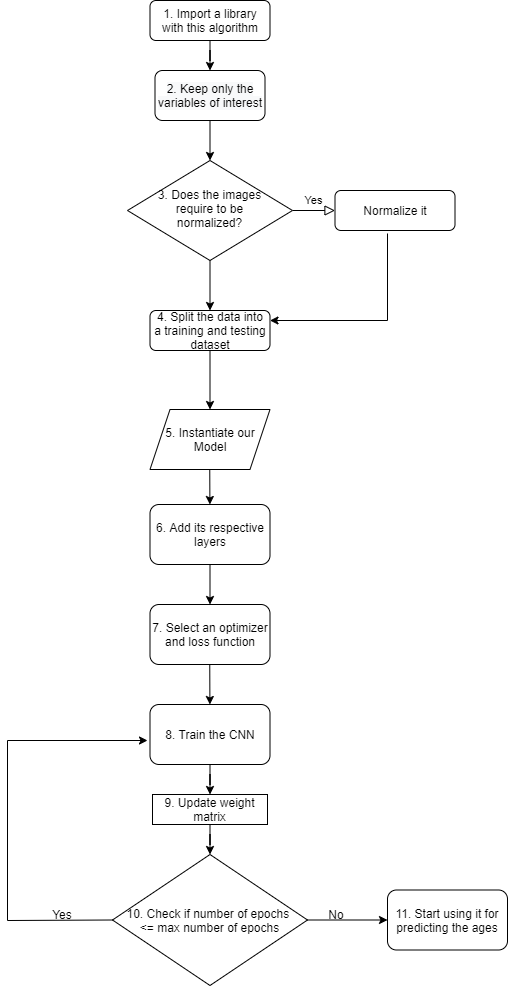
\includegraphics{img/CNN_algorithm_flowchart.png}

    \hypertarget{legend}{%
\subsubsection*{Legend:}\label{legend}}

    \begin{enumerate}
\def\labelenumi{\arabic{enumi}.}
\tightlist
\item
  In this case, Tensorflow could be used for implementing the CNN,
  especifically the Keras API
\item
  As the algorithm will obtain the features it requires from the images
  and the age is the target variable, we only need to keep the path to
  the images and the age in this step
\item
  Normalizing the scale of the images (rescaling its pixel values to be
  between 0 and 1) is usually required for having better predictions.
  However, there are cases in which the data is already normalized, so
  checking this becomes necessary
\item
  In order to train and validate our model, we require to split our data
  into a training and testing dataset.
\item
  We have to choose which model we want to instantiate. If Keras is
  being used, this implies choosing between a Sequential (linear stack
  of layers) and a Functional (arbitrary graph of layers) model. In this
  case, the Sequential will be used because its the simplest one
\item
  We will add 3 layers.

  \begin{enumerate}
  \def\labelenumii{\arabic{enumii}.}
  \tightlist
  \item
    A layer to specify the input shape, (i.e.~Conv2D)
  \item
    Another layer to pool the data (i.e.~MaxPooling2D)
  \item
    A final layer to give the model the ability to make predictions
    (i.e.~softmax)
  \end{enumerate}
\item
  A method of optimization to find the best parameters for the model has
  to be defined. For instance, we could use Adam, a gradient-based one.
  In addition, a loss function has to be specified, like the sparse
  categorical crossentropy, which is used for multiclass classification
  of mutually exclusive classes.
\item
  Train the model using the training data
\item
  After the multilayer model is trained, the previous value of its
  weight matrix will be updated
\item
  We will make our model work through the training data an specific
  number of times (= max number of epochs)
\item
  Finally, we can start making predictions with our updated model
\end{enumerate}

    \hypertarget{training-the-cnn}{%
\subsubsection*{Training the CNN}\label{training-the-cnn}}

    Fitting the model only requires inputting the training dataset (images
and ages), the number of epochs and the batch size to the Keras
\texttt{fit} command

    \hypertarget{testing-the-cnn}{%
\subsubsection*{Testing the CNN}\label{testing-the-cnn}}

    The model can be evaluated using the command \texttt{evaluate}, which
uses our fitted model in the testing dataset


    % Add a bibliography block to the postdoc
    
    
    
\end{document}
